% ------ ML process overview figure

\begin{tikzpicture}
\node[inner sep=0pt] (mlProcess) at (-2.1,0) {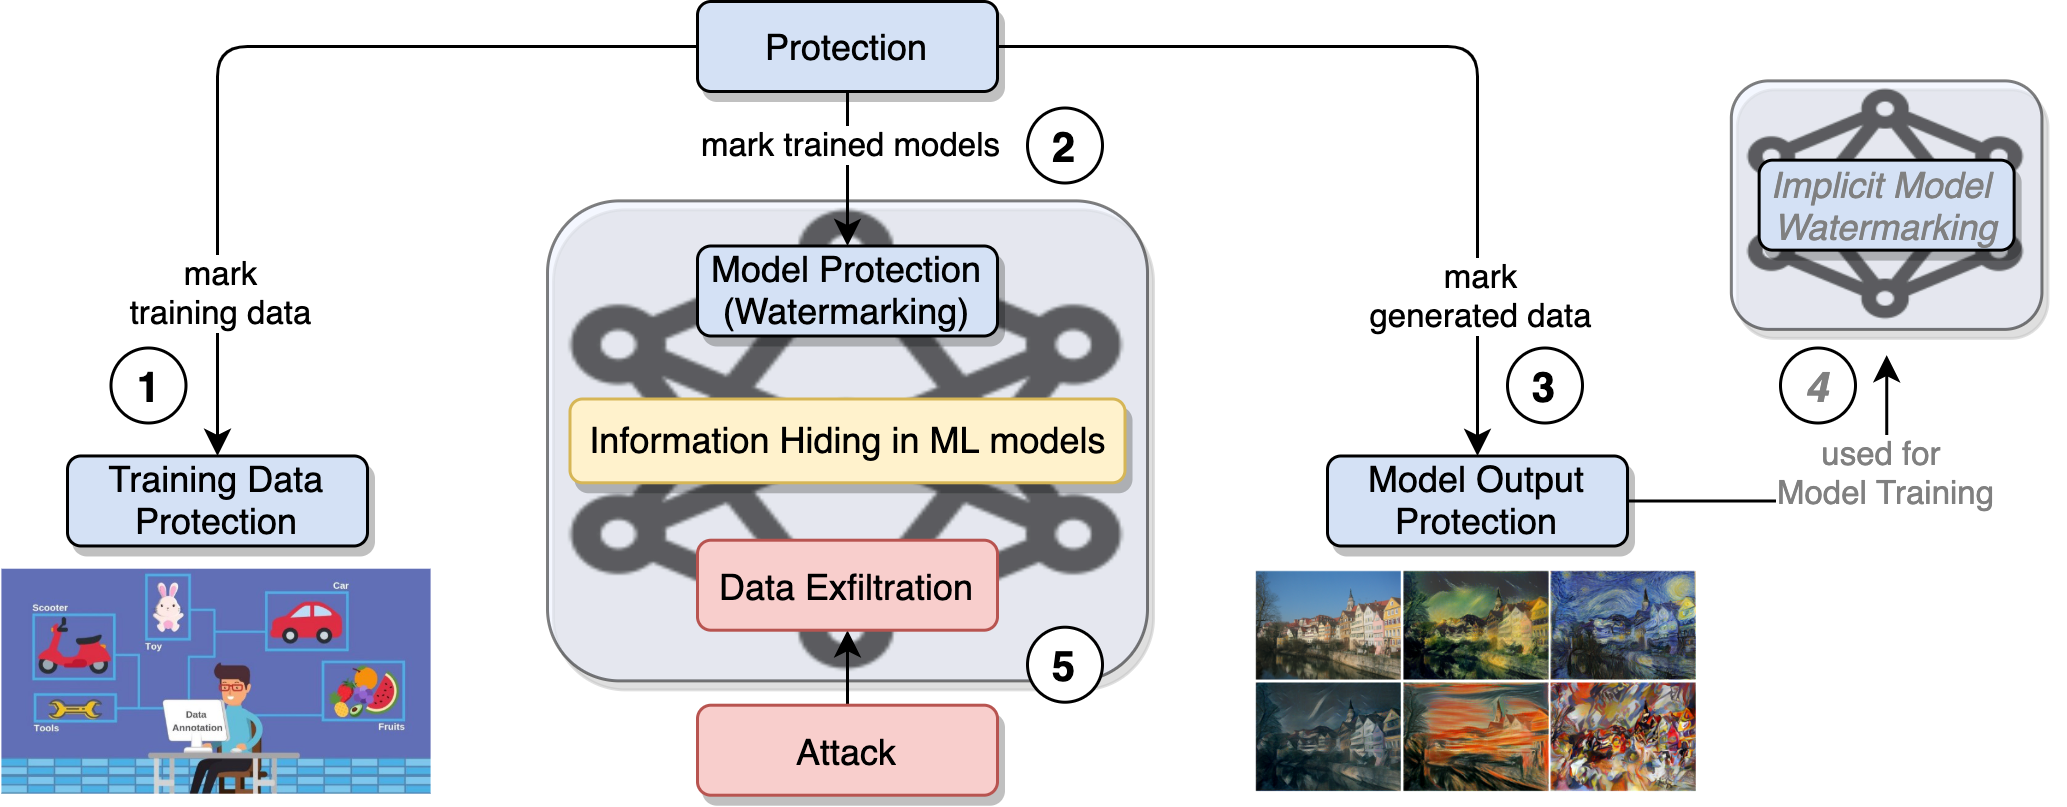
\includegraphics[width=\linewidth]{images/Watermarking_aspects.png}};

%MarkTrainingData:
\node[inner sep=0pt] (cite200) at (-7.5,0.1) {\tiny \cite{sablayrolles_radioactive_2020}};
%MarkOutputData:
% marks output, doesn't talk about model training
\node[inner sep=0pt] (cite211) at (0.7,0.1) {\tiny \cite{abdelnabi_adversarial_2020}};

%specifically for model training!
\node[inner sep=0pt] (cite212) at (4.5,0.35) {\tiny \cite{szyller_dawn_2020}};

% marks all output for surrogate model training
\node[inner sep=0pt] (cite213) at (4.5,0.1) {\tiny \cite{zhang_model_2020}};
\node[inner sep=0pt] (cite214) at (4.5,-0.15) {\tiny \cite{wu_watermarking_2020}};
%OtherInformationHiding
\node[inner sep=0pt] (cite225) at (-2.5,-1.8) {\tiny \cite{song_machine_2017}};
\end{tikzpicture}